\documentclass{article}
\newtheorem{thm}{Theorem}
\setlength{\oddsidemargin}{0.25in}
\setlength{\textwidth}{6in}
\setlength{\topmargin}{-0.25in}
\setlength{\headheight}{0.3in}
\setlength{\headsep}{0.2in}
\setlength{\textheight}{9in}
\setlength{\footskip}{0.1in}
\usepackage{multirow}
\usepackage{fullpage}
\usepackage{graphicx}
\usepackage{amsthm}
\usepackage{amssymb}
\usepackage{url}
\usepackage{amsfonts}
\usepackage{algpseudocode}
\usepackage{mathtools}
\newcommand{\quotes}[1]{``#1''}

\usepackage{hyperref}
\hypersetup{
    colorlinks=true,
    linkcolor=blue,
    filecolor=magenta,      
    urlcolor=blue,
}


\usepackage{listings}
\usepackage{xcolor} 

\lstset{numbers=left, 
	numberstyle=\tiny, 
	keywordstyle=\color{blue}, 
	commentstyle=\color[cmyk]{1,0,1,0}, 
	frame=single, 
	breaklines, 
	extendedchars=false, 
	xleftmargin=2em,xrightmargin=2em, aboveskip=1em, 
	tabsize=4, 
	showspaces=false 
}

\begin{document}\title{Homework 4\\ Introduction to Data Analysis and Mining \\ Spring 2018\\ CSCI-B 365}         % Enter your title between curly braces
\author{Siyi Xian}        % Enter your name between curly braces
\date{March 18, 2018}          % Enter your date or \today between curly braces
\maketitle
\makeatother     % `@' is restored as a "non-letter" character
\pagestyle{plain}
All the work herein is solely mine.
\section*{Directions}
Please follow the syllabus guidelines in turning in your homework.  I am providing the \LaTeX{} of this document too. This homework is due Tuesday, March  20, 2018 10:00p.m. \textbf{OBSERVE THE  TIME}. Absolutely no homework will be accepted after that time. All the work should be your own.  
 
   %%%%%%%%%%%%%%%%%%%%%%%%%%%%%%%%%%%%%%
%                      PROBLEM 1
 %%%%%%%%%%%%%%%%%%%%%%%%%%%%%%%%%%%%%%


  \section*{Problem 1 [30 points]}  
  
In this question, you will first perform principal component analysis (PCA) over  \href{https://archive.ics.uci.edu/ml/datasets/ionosphere}{
Ionosphere Data Set} and then cluster the  reduced data using your $k$-means program ($C_k)$ from previous homework. You are allowed to use R packages for PCA and ignore the class variables (35th variable) while performing PCA. Answer the questions below:
 \\
  \begin{enumerate}
  \item[\textbf{1.1)}] Perform PCA over Ionosphere data set and make a of PC1 and PC2 (the first two principal components). Are PC1 and PC2 linearly correlated?  
 \\
  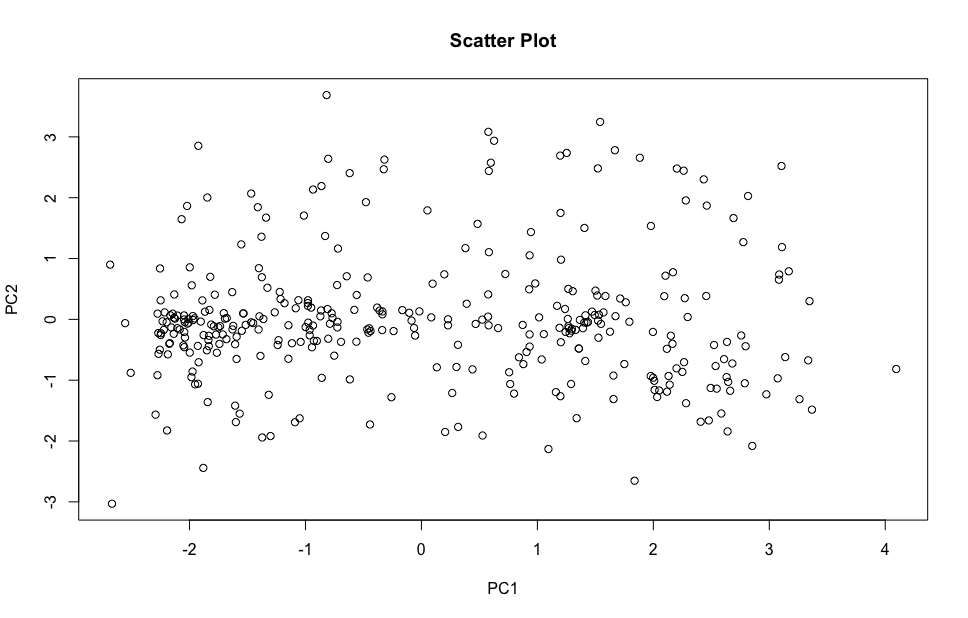
\includegraphics[width=10cm]{1-1-prcomp.png}
  \begin{verbatim}
  PC1 and PC2 are uncorrelation
  \end{verbatim}
\pagebreak

  \item[\textbf{1.2)}]  There are three methods to pick the set of principle components: (1) In the plot where the curve bends; (2)
Add the percentage variance until total $75\%$ is reached ($70-90\%$) (3) Use the components whose variance
is at least one. Show the components selected in the Ionosphere data  if each of these is used.
\\

\begin{lstlisting}[language = R]
# Please see specific claculation in pca1.R
> i
[1] 9
\end{lstlisting}

  \item[\textbf{1.3)}]  Observe the loadings using prcomp() or princomp() functions in R and  discuss loadings in PCA?i.e., how are principal components and original variables related?
\\
\begin{verbatim}
When using pca$rotation * pca$x, we can get a result that is similar to the origin data. 
So the loadings are items that connect PC and original variables.
\end{verbatim}


  \item[\textbf{1.4)}] Perform dimensionality reduction over Ionosphere data set with PCA.  Keep $90\%$ of variance  after PCA and reduce Ionosphere data set and call this data $\Delta_R$. Cluster  $\Delta_R$ using your $k$-means program from previous assignment and report the total error rates for $k = 2,\ldots,5$ for 20 runs each. Plots are generally a good way to convey complex ideas quickly, i.e., box plots, whisker plots. Discuss your results, i.e how did PCA affect  performance of $k$-means clustering.
  
  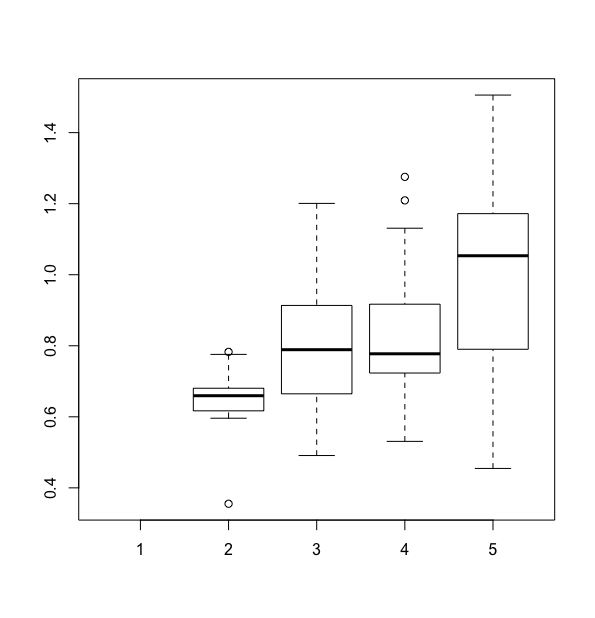
\includegraphics[width=4cm]{1-4.png}
  \begin{verbatim}
  This is the box plot after keeping 90% variance
  \end{verbatim}
  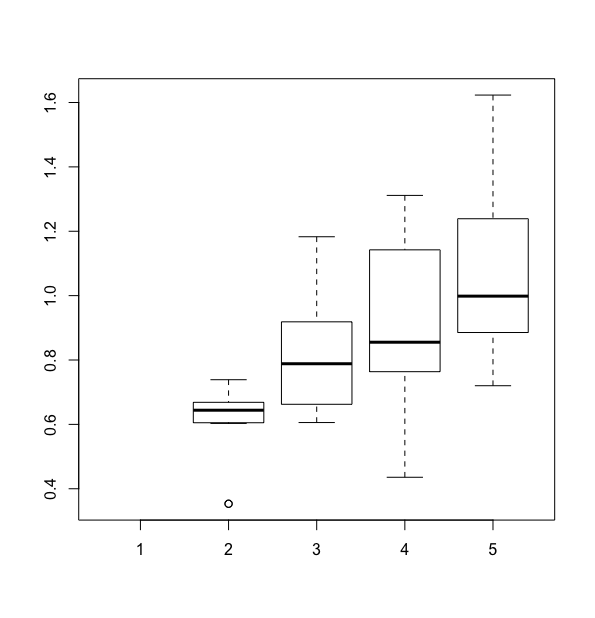
\includegraphics[width=4cm]{1-4-1.png}
  \begin{verbatim}
  This id the box plot with orrigin data points
  \end{verbatim}
  
  \begin{verbatim}
  According to the difference between two box plot, we can find out that the error rate 
  is increasing a little bit but all other parts are remain similarly. So I think that
  after reduce component based on PCA, the K-means algorithm is istill working kind of 
  good. 
  \end{verbatim}
\end{enumerate}  


\pagebreak
  %%%%%%%%%%%%%%%%%%%%%%%%%%%%%%%%%%%%%%
%                      PROBLEM 2
 %%%%%%%%%%%%%%%%%%%%%%%%%%%%%%%%%%%%%%
 \section*{Problem 2 [30 points]}  Randomly choose 50 points from Ionosphere data set (call this data set $\text{I}_{50}$) and perform hierarchical clustering. You are allowed to use R packages for this question. (Ignore the class variable while performing hierarchical clustering.)
 \\ 
 
 \begin{enumerate}
  \item[\textbf{2.1)}]  Using hierarchical clustering with complete linkage and Euclidean distance cluster $\text{I}_{50}$. Give the dendrogram.
\\ 
 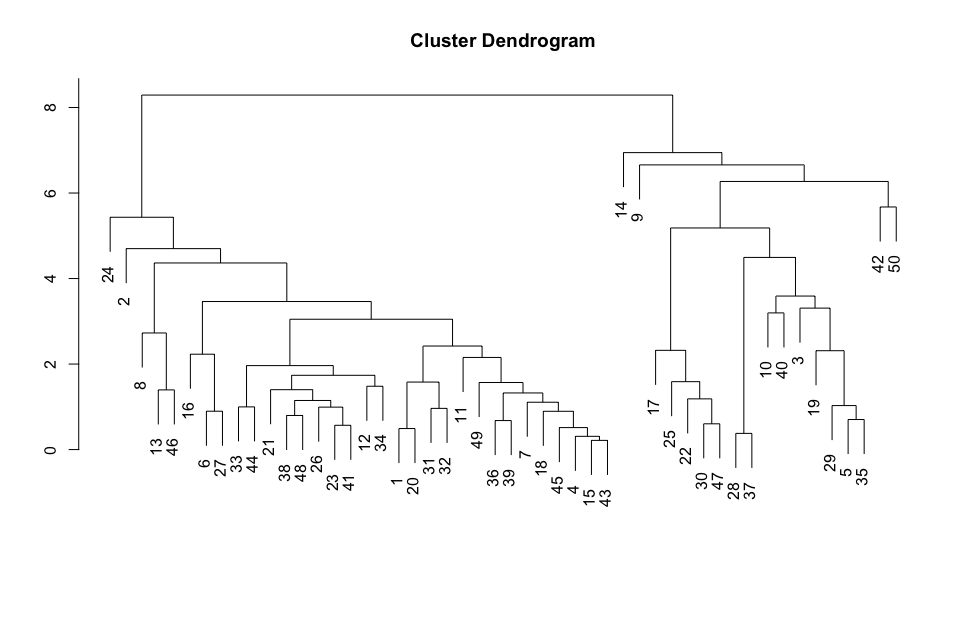
\includegraphics[width=10cm]{2-1.png}
 
\item[\textbf{2.2)}] Cut the dendrogram at a height that results in two distinct  clusters. Calculate the error-rate.
\\  

\begin{lstlisting}[language=R]
# Please see detailed code in hierarchical2.R file
> error_rate1
[1] 0.09375
> error_rate2
[1] 0.5
\end{lstlisting}

  \item[\textbf{2.3)}] First, perform PCA on $\text{I}_{50}$ (Keep $90\%$ of variance ). Then hierarchically cluster the reduced data using complete linkage and Euclidean distance. Report the dendrogram.
\\  
  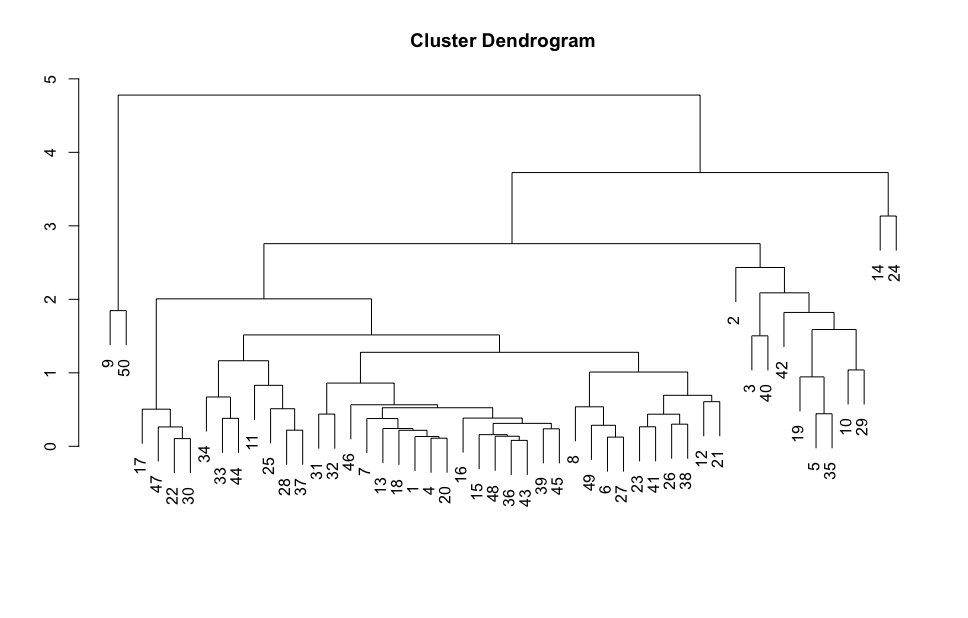
\includegraphics[width=10cm]{2-3.png}
  \pagebreak
    \item[\textbf{2.4)}]  Cut the dendrogram at a height that results in two distinct  clusters. Give the error-rate.  Discuss your findings, i.e., how  did PCA affect hierarchical clustering results?
    \begin{lstlisting}[language=R]
    # Please see detailed code in hierarchical2.R file
    > error_rate1
    [1] 0.2083333
    > error_rate2
    [1] 0
    \end{lstlisting}
    \begin{verbatim}
    Although we get the error rate reduced, we still meet a problem that one of the 
    cluster only have two points. The reason that although we keep 90% of variance, 
    first two columns of this data set is kind of usless, but we keep them. So that 
    is some problem which we need to improve when using PCA.
    \end{verbatim}
\end{enumerate}

\pagebreak
 %%%%%%%%%%%%%%%%%%%%%%%%%%%%%%%%%%%%%%
%                      PROBLEM 3
 %%%%%%%%%%%%%%%%%%%%%%%%%%%%%%%%%%%%%%
  \section*{Problem 3 [20 points]} 
From textbook, Chapter 8 exercises 16, 18 and 30 (Pages 563-566)
\begin{enumerate}
	\item[\textbf{16.}] Perform single and complete link hierarchical clustering.
	\\
	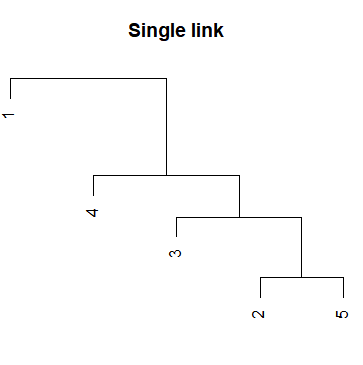
\includegraphics[width=7cm]{8-a.png}
	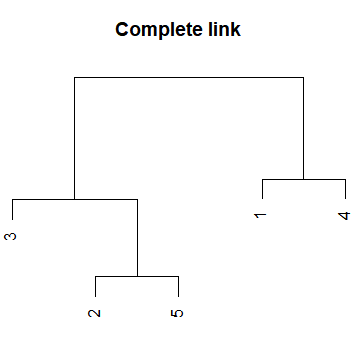
\includegraphics[width=7cm]{8-b.png}
	
	\item[\textbf{18.}] Suppose we find $K$ clusters using Ward’s method, bisecting K-means, and ordinary K-means. Which of these solutions represents a local or global minimum? Explain.
	\begin{verbatim}
	Although Ward's method using minimize SSE to choose clusters, it does not have maintine 
	step, which means that this method does not have any refinement step. As for bisecting 
	K-means, is also does not have any step about maintiness. Thus, does not like regular 
	K-means, either Wards's method and bisecting K-means do not have local minimum. However, 
	all the three methods cannot determain the global minimum. 
	
	
	\end{verbatim}
	
		
	\item[\textbf{30.}] Clusters of documents can be summarized by finding the top terms (words) for the documents in the cluster, e.g., by taking the most frequent $k$ terms, where $k$ is a constant, say 10, or by taking all terms that occur more frequently than a specified threshold. Suppose that K-means is used to find clusters of both documents and words for a document data set.
	\begin{enumerate}
		\item [\textbf{(a)}] How might a set of term clusters defined by the top terms in a document cluster differ from the word clusters found by clustering the terms with K-means?
		\begin{enumerate}
			\item [1)]
			\begin{verbatim}
			The top clusters might be overlapped.
			\end{verbatim}
			\item [2)]
			\begin{verbatim}
			There are possibility that some items may not shown by the top terms.
			\end{verbatim}
		\end{enumerate}
		\item [\textbf{(b)}] How could term clustering be used to define clusters of documents?
		\begin{verbatim}
		Take top documents as one term cluster.
		\end{verbatim}
	\end{enumerate}
\end{enumerate}


\pagebreak
 %%%%%%%%%%%%%%%%%%%%%%%%%%%%%%%%%%%%%%
%                   EXTRA CREDIT
 %%%%%%%%%%%%%%%%%%%%%%%%%%%%%%%%%%%%%%
  \section*{Extra Credit [10 points]} 

From textbook, Chapter 8 exercise 12 (Page 562).
\begin{enumerate}
	\item [\textbf{12.}] The leader algorithm (Hartigan [4]) represents each cluster using a point, known as a leader, and assigns each point to the cluster corresponding to the closest leader, unless this distance is above a user-specified threshold. In that case, the point becomes the leader of a new cluster.
	\\
	Note that the algorithm described here is not quite the leader algorithm described in Hartigan, which assigns a point to the first leader that is within the threshold distance. The answers apply to the algorithm as stated in the problem.
	\begin{enumerate}
		\item [\textbf{(a)}] What are the advantages and disadvantages of the leader algorithm as compared to K-means?
		\begin{enumerate}
			\item [Advantage:]
			\begin{enumerate}
			\item[1)] 
			\begin{verbatim}
			Require less data
			\end{verbatim}
			\item[2)] 
			\begin{verbatim}
			More efficiency
			\end{verbatim}
			\end{enumerate}
			\item [Disadvantage:]
			\begin{verbatim}
			Because Leader Algorithm is ordered, it will perduce same clusters every time. 
			However, for K-means, it can perduce better clusters when using SSE to 
			determine that.
			\end{verbatim}
		\end{enumerate}
		\item [\textbf{(b)}] Suggest ways in which the leader algorithm might be improved.
		\begin{verbatim}
		Adding thresholds when clustering data points.
		\end{verbatim}
	\end{enumerate}
\end{enumerate}


\pagebreak
%%%%%%%%%%%%%%%%%%%%%%%%%%%%%%%%%%%%%%
\section*{What to Turn-in}
 Submit a .zip file that includes the files below. Name the .zip  file as \quotes{usename-section number}, i.e., hakurban-B365.


\begin{itemize}
\item The *tex and *pdf of the written answers to this document.
\item *\texttt{R}files for:
\begin{itemize}
\item R code for problem 1 (\quotes{pca1.R}).
\item R code for problem 2 (\quotes{hierarchical2.R}).
\end{itemize}
\end{itemize}




\end{document}


